\documentclass[11pt]{article}
\usepackage{amsmath,amsthm,amsfonts,amssymb}
\usepackage[margin=1in]{geometry}
\usepackage{fancyhdr}
\usepackage{hyperref}
\usepackage{xcolor}
\usepackage{tcolorbox}

\usepackage{tcolorbox}
\usepackage{enumerate}
\usepackage{tikz}
\usetikzlibrary{arrows.meta, positioning}


\usepackage{algorithmic}

\usetikzlibrary{arrows.meta}

    \setlength{\headheight}{26pt}
    \pagestyle{fancy}
    \fancyhead[C]{\textbf{Basic Algorithms (Section 5)}\\Spring 2025}
    \fancyhead[R]{HW9 (Due 4/17 23:59)\\ Instructor: Jiaxin Guan}
    \fancyfoot[C]{}
    \fancyfoot[R]{\thepage}
    \renewcommand{\headrulewidth}{0.4pt}
    \renewcommand{\footrulewidth}{0.4pt}  
    

\begin{document}


    %%%% EDIT THIS PART 
    %Put your name and Net ID here
    \fancyhead[L]{Name: Nick Zhu \\ Net ID: xz4687}
    %Write your collaborators' names here
    \fancyfoot[L]{Discussion Partners: Ray Li}
    %%%%%

    %Problem 1
    \begin{tcolorbox}[title={Problem 1 (DFS Olympics, 30 pts)}] \setlength\parindent{1em}
        Consider running depth first search on a graph $G$ of $n$ nodes. As in lecture, for each vertex $v$ we will keep track of $\texttt{disc}[v]$ and $\texttt{finish}[v]$, the times when $v$ is first discovered and when $v$ finishes being processed respectively.

        For some graph $G=(V,E)$, we can consider $\max_{v \in V} \texttt{disc}[v]$ and $\max_{v \in V} \texttt{finish}[v]$, the largest values of $\texttt{disc}[v]$ and $\texttt{finish}[v]$ in the graph.

        \begin{enumerate}[(a)]
            \item Over all graphs $G=(V,E)$ of size $|V|=n$, what is the maximum value of $\max_{v \in V} \texttt{disc}[v]$? What is the minimum value? Give two graphs on $6$ vertices satisfying these two values respectively.
            
            \item Over all graphs $G=(V,E)$ of size $|V|=n$, what is the maximum value of $\max_{v \in V} \texttt{finish}[v]$? What is the minimum value? Give two graphs on $6$ vertices satisfying these two values respectively.
            
            \item Over all graphs $G=(V,E)$ of size $|V|=n$, what is the maximum value of $\max_{v \in V} (\texttt{finish}[v] - \texttt{disc}[v])$? What is the minimum value? Give two graphs on $6$ vertices satisfying these two values respectively.
        \end{enumerate}   
    \end{tcolorbox}
    
    %Write your solution here!
    \section*{Solution}

    \subsection*{(a)}
    The largest possible value of $\max_{v\in V}\,\texttt{disc}[v]$ is $2n-1$, and the smallest possible value is $n$.\\ 
    For $n=6$:
    \begin{itemize}
      \item \emph{Maximum:} the empty graph on 6 vertices.  DFS discovers each vertex in its own call, so the sixth discovery occurs at time $2\cdot6-1=11$.
      \item \emph{Minimum:} the directed path $1\to2\to3\to4\to5\to6$.  A single DFS call visits all vertices consecutively at discovery times $1,2,\dots,6$.
    \end{itemize}
    
    \subsection*{(b)}
    Over all directed graphs $G=(V,E)$ with $|V|=n$, every DFS performs exactly $n$ discoveries and $n$ finishes, so the very last finish happens at time $2n$.\\
    The maximum and minimum values of $\max_{v\in V}\,\texttt{finish}[v] = 2n$ in every case.  \\
    For $n=6$, in both the empty graph and the 6‑vertex path examples above (section (a)), the final finish time is $12$.
    
    \subsection*{(c)}
    The largest possible value of $\max_{v\in V}\bigl(\texttt{finish}[v]-\texttt{disc}[v]\bigr)$ is $2n-1$, and the smallest possible value is $1$.\\ 
    For $n=6$:
    \begin{itemize}
      \item \emph{Maximum:} the directed path $1\to2\to3\to4\to5\to6$.  Vertex 1 is discovered at time 1 and finishes at time 12, so its value of $\max_{v\in V}\bigl(\texttt{finish}[v]-\texttt{disc}[v]\bigr)$ is $11$.
      \item \emph{Minimum:} the empty graph.  Each vertex is discovered and then immediately finished, so its value of $\max_{v\in V}\bigl(\texttt{finish}[v]-\texttt{disc}[v]\bigr)$ is $1$.
    \end{itemize}

    \newpage
    %Problem 2
    \begin{tcolorbox}[title={Problem 2 (Failed Magic, 20 pts)}] \setlength\parindent{1em}
         In Lecture 17, we saw a magic trick that can turn a BFS algorithm into a DFS algorithm by simply replacing the queue with a stack. But I mentioned that this magic trick does not work for all BFS algorithms. In this problem, we will see why.

         Below is the BFS algorithm from Lecture 16, but with the queue replaced by a stack attempting to make it into a DFS. Find a counterexmaple, i.e. construct a graph $G=(V,E)$ (can be either directed or undirected), such that for some vertex $s\in V$, running $\textsc{DFS-Visit}(G, s)$ does not correctly give you a DFS tree. The issue is with \textbf{the sequence of vertices} that you visit, so you may safely ignore the \textcolor{teal}{teal}-colored lines for the distances, as they are not used for DFS.

         You should specify the graph $G$ (drawing it out is fine) and the vertex $s$ that you run DFS on, along with a quick explanation of what goes wrong with the (incorrect) DFS tree it produces. (\emph{Hint: A simple example only needs 3 vertices.})

        
        \par\noindent\rule{\textwidth}{0.4pt}
        \smallskip        
        \textsc{DFS-Visit}$(G,s)$
        \begin{algorithmic}[1]
            \FOR{all $v\in V$}
                \STATE \textcolor{teal}{$\texttt{dist}(v)\gets \infty$}
                \STATE $\texttt{parent}(v)\gets \bot$
                \STATE $\texttt{color}(v)\gets \texttt{WHITE}$
            \ENDFOR
            \STATE \textcolor{teal}{$\texttt{dist}(s)\gets 0$}
            \STATE $\texttt{color}(s)\gets \texttt{YELLOW}$
            \STATE $\textsf{Stack}.\texttt{push}(s)$
            \WHILE{\textsf{Stack} is not empty}
                \STATE $u\gets \textsf{Stack}.\texttt{pop}()$
                \FOR{all $v \in \mathsf{Adj}[u]$}
                \IF{$\texttt{color}(v)=\texttt{WHITE}$}
                    \STATE \textcolor{teal}{$\texttt{dist}(v)\gets \texttt{dist}(u)+1$}
                    \STATE $\texttt{parent}(v)\gets \texttt{u}$
            \STATE $\texttt{color}(v)\gets \texttt{YELLOW}$
            \STATE $\textsf{Stack}.\texttt{push}(v)$
                \ENDIF
                \ENDFOR
                \STATE $\texttt{color}(u)\gets \texttt{GREEN}$
            \ENDWHILE
        \end{algorithmic}
        \vspace{-2mm}
        \par\noindent\rule{\textwidth}{0.4pt}
    \end{tcolorbox}

    %Write your solution here!
    \section*{Solution}
    
    Consider the directed graph
    \[
      G = \bigl(\{1,2,3\},\;\{(1,2),\,(2,3),\,(1,3)\}\bigr)
    \]
    \begin{figure}[h]
        \centering
        \begin{tikzpicture}[
            ->,                                % make all edges directed
            >=Stealth,                        % arrow tip style
            node distance=2cm,                % default distance between nodes
            every node/.style={circle,draw}  % style for all nodes
          ]
          \node (v1) {1};
          \node (v2) [right=of v1] {2};
          \node (v3) [below=of v2] {3};
        
          \draw (v1) -- (v2);
          \draw (v1) -- (v3);
          \draw (v2) -- (v3);
        \end{tikzpicture}
        \end{figure}
    and let the start vertex be \(s=1\).  Its adjacency lists are
    \[
      \mathrm{Adj}(1)=\{2,3\},\quad
      \mathrm{Adj}(2)=\{3\},\quad
      \mathrm{Adj}(3)=\emptyset.
    \]
    A true DFS from \(1\) (visiting neighbors in numerical order) explores
    \[
      1 \to 2 \to 3,
    \]
    producing \(\mathrm{parent}(2)=1\) and \(\mathrm{parent}(3)=2\).\\
    
    The $\textsc{DFS-Vist}(G,s)$ does the following:
    
    \begin{enumerate}
      \item Push \(1\).
      \item Pop \(1\); scan \(\{2,3\}\): push \(2\), then push \(3\).
      \item Pop \(3\) next (LIFO!), set \(\mathrm{parent}(3)=1\).
      \item Pop \(2\) last; when scanning \(\{3\}\), vertex 3 is already non‑white, so no change.
    \end{enumerate}
    
    This (incorrect) “DFS tree” has edges \((1,2)\) and \((1,3)\), whereas the correct DFS tree has edges \((1,2)\) and \((2,3)\).  Hence this 3‑vertex graph is a counterexample. 
   
    \newpage
    %Problem 3
    \begin{tcolorbox}[title={Problem 3 (Cycle Detection, 20 pts)}] \setlength\parindent{1em}
         Explain how to modify an algorithm from class to detect if an undirected graph $G=(V,E)$ has a cycle in time $O(|V|)$ (independent of the number of edges). Justify the correctness and runtime of your proposed algorithm. 
         
         (\textit{Hint: Something from the last homework might come handy})
    \end{tcolorbox}
    
    %Write your solution here!
    \section*{Solution}

    We first test the edge count:
    
    \begin{itemize}
      \item If \(\lvert E\rvert \ge \lvert V\rvert\), then any undirected forest on \(\lvert V\rvert\) vertices can have at most \(\lvert V\rvert-1\) edges.  Hence in \(O(1)\) time we conclude “cycle.”
      \item Otherwise \(\lvert E\rvert<\lvert V\rvert\), so we run the usual DFS
      \begin{itemize}
        \item Initially, for every \(v\in V\), set \(\texttt{color}(v)\gets\texttt{WHITE}\).
        \item On first visiting \(u\), set \(\texttt{color}(u)\gets\texttt{YELLOW}\).
        \item After all neighbors of \(u\) are processed, set \(\texttt{color}(u)\gets\texttt{GREEN}\).
        \item When exploring an edge \(\{u,v\}\):
          \begin{itemize}
            \item If \(\texttt{color}(v)=\texttt{WHITE}\), recurse on \(v\).
            \item If \(\texttt{color}(v)=\texttt{YELLOW}\) and \(v\neq\texttt{parent}(u)\), then \(\{u,v\}\) is a backward edge in an undirected DFS, so we immediately conclude “cycle.”
          \end{itemize}
      \end{itemize}
    \end{itemize}
    
    \paragraph{Correctness.}  
    We consider two cases:
    
    \begin{description}
      \item[Case 1: \(\lvert E\rvert \ge \lvert V\rvert\).]  
        A classical fact about forests is that a connected, acyclic undirected graph on \(n\) vertices has exactly \(n-1\) edges, and in general a forest on \(n\) vertices has at most \(n-1\) edges.  Thus if \(\lvert E\rvert \ge \lvert V\rvert\), no matter how the edges are arranged, the graph cannot be acyclic.  Concluding “cycle” in this case is therefore always correct.
    
      \item[Case 2: \(\lvert E\rvert < \lvert V\rvert\).]  
        Here we run the usual DFS cycle‐detection.  In an undirected graph, a cycle exists if and only if DFS ever encounters a “backward edge”—an edge \(\{u,v\}\) leading to a vertex \(v\) that is currently in the recursion stack (\(\texttt{YELLOW}\)) but is not the immediate parent of \(u\).  No backward‐edge test can ever give a false positive (every such edge closes a cycle), and every cycle in the graph must eventually produce at least one backward edge in some DFS tree.  Since we perform this test exhaustively over all reachable vertices, we will detect a cycle exactly when one exists.
    \end{description}
    
    \paragraph{Runtime.}  
    \begin{itemize}
      \item The check \(\lvert E\rvert \ge \lvert V\rvert\) takes \(O(1)\) once \(\lvert E\rvert\) is known.  (If the edge list is stored explicitly, counting \(\lvert E\rvert\) is \(O(1)\) if provided, or \(O(\lvert E\rvert)\) to scan once; but since we only enter DFS when \(\lvert E\rvert<\lvert V\rvert\), even that initial scan is \(O(\lvert V\rvert)\).)
      \item In the case \(\lvert E\rvert<\lvert V\rvert\), we run DFS on an adjacency‐list representation.  DFS takes \(O(\lvert V\rvert + \lvert E\rvert)\) time.
        Since here \(\lvert E\rvert<\lvert V\rvert\), we have
        \[
          O(\lvert V\rvert + \lvert E\rvert) \;=\; O(\lvert V\rvert + \lvert V\rvert - 1)\;=\;O(\lvert V\rvert).
        \]
    \end{itemize}
    
    Combining both cases, the entire procedure runs in \(O(\lvert V\rvert)\) time, independent of the original edge count.
    
    \newpage
    %Problem 4
    \begin{tcolorbox}[title={Problem 4 (Number of Simple Paths, 30 pts)}] \setlength\parindent{1em}
        Give an algorithm that given a Directed Acyclic Graph (DAG, defined as a directed graph without cycles) and two vertices $s,t$, returns the \emph{number} of simple paths from $s$ to $t$. Your algorithm should run in time $O(|V|+|E|)$. Justify the correctness and runtime of your proposed algorithm. (Your algorithm does not need to list the simple paths, only needs to give the count.)

        (\emph{Hint: What is the letter after C? What is the letter before Q?})
    \end{tcolorbox}
    %Write your solution here!
    \section*{Solution}

    \par\noindent\rule{\textwidth}{0.4pt}
    \smallskip
    \textsc{CountPaths}$(G=(V,E),\,s,\,t)$
    \begin{algorithmic}[1]
        \STATE Compute a topological ordering of $V$, store it in list $L$
        \FOR{each $v\in V$}
            \STATE $\mathit{dp}[v]\gets 0$
        \ENDFOR
        \STATE $\mathit{dp}[s]\gets 1$
        \FOR{each $u$ in $L$ (in topological order)}
            \FOR{each $v\in \mathrm{Adj}(u)$}
                \STATE $\mathit{dp}[v]\gets \mathit{dp}[v] + \mathit{dp}[u]$
            \ENDFOR
        \ENDFOR
        \STATE \textbf{return} $\mathit{dp}[t]$
    \end{algorithmic}
    \vspace{-2mm}
    \par\noindent\rule{\textwidth}{0.4pt}
    
    \paragraph{Correctness.}  
    Since $G$ is a DAG, a topological order $L$ exists.  We maintain the invariant that $\mathit{dp}[v]$ equals the number of simple paths from $s$ to $v$ using only vertices earlier than or equal to $v$ in $L$.  Initially only $s$ has $\mathit{dp}[s]=1$.  When we process $u$, all contributions from paths ending at $u$ have been accumulated, so propagating $\mathit{dp}[u]$ along each outgoing edge correctly adds all new paths to each successor.  Because there are no cycles, each simple path from $s$ to $t$ is counted exactly once.
    
    \paragraph{Runtime.}  
    Topological sorting runs in $O(|V|+|E|)$.  Initializing the $\mathit{dp}$ array takes $O(|V|)$, and the nested loops over each vertex in $L$ and its outgoing edges take $O(|E|)$.  Hence the total time is
    \[
      O(|V|+|E|).
    \]

\end{document}